\def\notedate{2022.02.09}
\def\currentauthor{Тришин И.В. (РК6)}%
%----------------------------------------------------------
\notestatement{rndhpcblo}{Сравнительная характеристика GBSE, pSeven, Pradis}

В рамках сравнения были рассмотрены известные программные комплексы, в основе которых в том или ином виде лежит идея организации вычислений, описываемая с помощью ориентированных графов (графоориентированный подход).

Для проведения сравнения с программным каркасом GBSE выбирались программные продукты, в которых так или иначе реализован описанный выше подход. В первую очередь был рассмотрен программный комплекс pSeven, разработанный отечественной компанией DATADVANCE. Он направлен в первую очередь на решение конструкторских, оптимизационных задач и, помимо этого, задач анализа данных, что в первом приближении делает его аналогом GBSE по предметному назначению. У автора работы присутствует опыт работы с этим комплексом в рамках прохождения курса лабораторных работ по изученной на кафедре дисциплине "Методы оптимизации". В данном курсе были освещены основы работы с pSeven и основные приниципы организации вычислений в нём. Таким образом, на момент выбора программных комплексов для сравнения уже имелась некоторая информация о pSeven, которая позволила включить его в рассмотрение.

Кроме того, научным руководителем данной работы была рекомендована разработка отечественной компании ``Ладуга'' PRADIS - комплекс, так же направленный на решение конструкторских задач. В данной разработке основной упор сделан на задачи анализа проектных решений на микро- и макроуровне.

\subsubsection{Выделение признаков для сравнения}

% При выделении сравнительных признаков необходимо было, чтобы они охватывали достаточно широкую область сведений о программном продукте.

Среди прочих должны были быть выделены признаки, относящиеся как к общей структуре программного комплекса, так и к особенностям реализации в нём графоориентированного подхода и, кроме того, к особенностям взаимодействия с пользователем при решении задач, требующих действий с его стороны.

Сравнение осуществлялось с учётом следующих характерных признаков:
\begin{enumerate}[label=\arabic*)]
    \item предметное назначение;
    \item принципы формирования графовых моделей;
    \item формат описания графовых моделей;
    \item файловая структура проекта проведения анализа \gls{TO};
    \item особенности работы с входными и выходными данными графовых моделей;
    \item особенности передачи данных между узлами графовых моделей;
    \item поддержка ветвлений и циклов в топологии графовых моделей;
    \item поддержка параллельной обработки данных;
    \item возможность выбрать из набора однотипных промежуточных результатов расчётов некоторые экземпляры и продолжить расчёт только для них;
    \item возможность доопределять входные данные непосредственно во время обхода графовой модели.
\end{enumerate}

\subsubsection{Программный комплекс Pradis}

Программный комплекс \textsf{Pradis}, разработанный отечественной компанией <<Ладуга>>, предназначен для анализа динамических процессов в системах разной физической природы (механических, гидравлических и т.д.). Как правило, при помощи данного комплекса решаются нестационарные нелинейные задачи, в которых характеристики системы зависят от времени и пространственных координат. Круг задач, которые могут быть решены с помощью \textsf{Pradis}, достаточно широк: возможен анализ любых технических объектов, модели поведения которых представимы системами обыкновенных дифференциальных уравнений (СОДУ). Анализ статических задач обеспечивается как частный случай динамического расчета.

Практические возможности по решению конкретных задач определяются текущим составом библиотек комплекса, прежде всего библиотек моделей элементов~\cite{PradisGeneral2007}.\pdfcomment{Было бы хорошо представить подробнее информацию о понятии 'модель': что это, как она представляется и пр.} Данный копмплекс был рекомедован к обзору и сравнению, однако, после проведённого обзора официальной документации~\cite{PradisMethods2007} не было получено достаточного представления об использовании элементов графоориентированных подходов в данном копмлексе, поэтому было принято решение исключить его из дальнейшего рассмотрения.

\subsubsection{Программный комплекс pSeven}

В программном комплексе \textsf{pSeven}, разработанном компанией DATADVANCE, используется методология диаграмм потоков данных (англ.~Dataflow diagram, DFD). В комплексе применяются ориентированные графы (орграфы) для описания процесса решения некоторой задачи проектирования технического объекта. В терминах \textsf{pSeven}: графовое описание процесса решения задачи называется \textit{расчетной схемой} (англ.~workflow), что, помимо прочего, соответствует классическому термину из области математического моделирования; узлам орграфа поставлены в соответствие процессы обработки данных (используется термин \textit{блоки}), а рёбра определяют \textit{связи} между блоками и направления передачи данных между процессами \cite{Nazarenko2015}. 

%...., определяется только зависимостями между входными и выходными данными каждого отдельного процесса их обработки, входящиего в решение . 
Используются следующие базовые понятия \textsf{pSeven}:
\begin{itemize}
    \item \textsf{расчётная схема} -- формальное описание процесса решения некоторой задачи в виде орграфа;
    \item \textsf{блок} -- программный контейнер для некоторого процесса обработки данных, входные и выходные данные для которого задаются через порты (см. ниже);
    \item \textsf{порт} -- переменная конкретного\footnote{Динамическая типизация не поддерживается.} типа, определённая в блоке и имеющая уникальное имя в его пределах;
    \item \textsf{связь} -- направленное соединение типа ``один к одному'' между выходным и входным портами разных блоков.
\end{itemize}

С учётом данных понятий можно описать используемую методологию диаграмм потов данных следующим образом. Расчётная схема содержит в себе набор процессов обработки данных (блоков), каждый из которых имеет (возможно, пустой) набор именованных входов и выходов (портов). Данные передаются через связи. Для избежания т.н. гонок данных (англ. data races) множественные связи с одним и тем же входным портом не поддерживаются. Для начала выполнения каждому блоку требуются данные на всех входных портах. Все данные на выходных портах формируются по завершении исполнения блока \cite{Nazarenko2015}.

\begin{figure}[h]
    \centering
    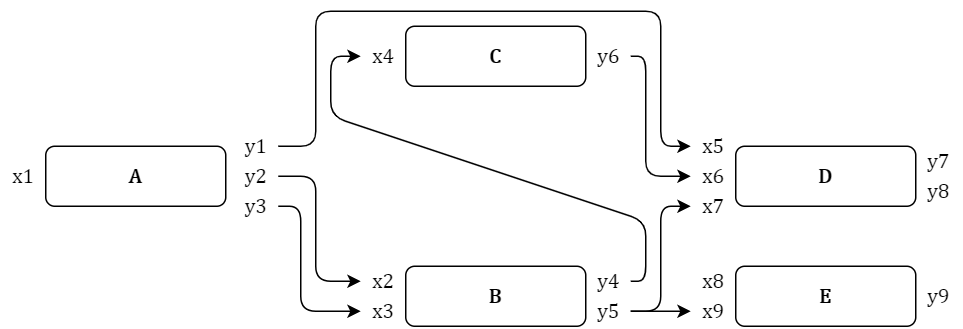
\includegraphics[width=\textwidth]{ResearchNotes/rndhpc_not_blo_2022_02_09/dataflow.png}
    \caption{Пример диаграммы потоков данных}
    \label{fig:dataflow}
\end{figure}

На рисунке \ref{fig:dataflow} $A, B, C, D$ - блоки обработки информации, $x_i$ - входные порты, $y_i$ - выходные. Стрелками показаны связи. Согласно изложенному выше принципу, сначала будет запущен блок $A$, по его завершении - блок $B$. Затем - блоки $C$ и $E$ (параллельно). По завершении блока $C$ будет запущен блок $D$. На этом обход расчётной схемы завершится, и значения $y_7, y_8$ и $y_9$ будут сохранены в локальной базе данных.

\begin{remark}[принцип обхода в pSeven]
Все порты, которые не привязаны к другим блокам, автоматически становятся внешними входами и выходами для всей расчётной схемы. Для начала обхода расчётной схемы должен быть предоставлен набор входных данных и указаны внешние выходные порты, значения которых обязательно должны быть вычислены в результате обхода. Обход производится в несколько этапов: сперва отслеживаются пути от необязательных выходных портов к входным, все встреченные на пути блоки помечаются, как неактуальные и не будут выполнены в дальнейшем; затем отслеживаются пути от обязательных выходных портов к входным и все встреченные на пути блоки помечаются, как обязательные к исполнению. Наконец, обязательные к исполнению блоки запускаются, начиная с тех, которые подключены к внешним входам расчётной схемы, а неактуальные игнорируются. Обход прекращается, когда не остаётся необходимых для выполнения блоков \cite{Nazarenko2015}. 
\end{remark}

По завершении обхода расчётной схемы результаты расчётов сохраняются в локальной базе данных проекта. В pSeven встроен инструментарий для визуализации и анализа результатов. Схемы, графики, гистограммы и результаты анализа сохраняются в т.н. отчётах - специальных файлах, сохраняемых в директории проекта.

\begin{landscape}

Результаты проведённого сравнения представлены в таблице \ref{rndhpcblo.0209}.

\begin{longtable}{|p{0.025\textwidth}|p{0.2\textwidth}|p{0.5\textwidth}|p{0.5\textwidth}|}
    \caption{Сравнительная таблица}\label{rndhpcblo.0209} \\
    \hline
    \textbf{№} & \textbf{Признак} & \textbf{pSeven} & \textbf{GBSE} \\
    \hline
    1 & Предметное назначение & Задачи оптимизации, анализ данных & Задачи автоматизированного проектирования, алгоритмизация сложных вычислительных методов, анализ данных \\
    \hline
    2 & Принцип формирования графовых моделей & Узлы -- блоки (процессы), рёбра -- связи (направление передачи данных) \cite{Nazarenko2015}. & Узлы -- состояния данных, рёбра -- переходы между состояниями, с указанием функций перехода \cite{SokPersh2018GBSE}. \\
    \hline
    3 & Формат описания орграфа & Расчетная схема (в форме орграфа) сохраняется в двоичный файле закрытого формата с расширением \textsf{.p7wf}. & Графовая модель (определяет алгоритм проведения комплексных вычислений в форме орграфа) сохраняется в текстовом файле открытого формата, подготовленного на языке \gls{aDOT}\cite{SokADOT}, являющегося ``сужением'' (частным случаем) известного формата DOT (Graphviz). \\
    \hline
    4 & Файловая структура проекта проведения анализа \gls{TO} & Проект состоит из непосредственно файла проекта, в котором хранятся ссылки на созданные расчётные схемы и локальную базу данных, сами расчётные схемы, файлы с их входными данными, файлы отчётов, где сохраняются выходные данные последних расчётов и результаты их анализа. & Проект состоит из \textsf{.aDOT} файла с описанием графа, \textsf{.aINI}-файлов с описанием форматов входных данных, библиотек функций-обработчиков, функций-предикатов и функций-селекторов , файлов, куда записываются выходные данные. \\
    \hline
    5 & особенности работы с входными и выходными данными графовых моделей & Входные данные должны быть указаны при настройках внешних входных портов расчётной схемы. Данные с выходных портов схемы сохраняются в локальной базе данных. Для их записи в файлы для обработки/анализа вне pSeven необходимо воспользоваться специально предназначенными для этого блоками. & Входные данные хранятся в файле в формате \gls{aINI}\cite{SokAINI}, откуда считываются при запуске обхода графа~\cite{SokPersh2017}. Для записи выходных/промежуточных данных в файлы или базы данных необходимо добавить соответствующие функции-обработчики. Формат выходных данных не регламентирован. \\
    \hline
    6 & Особенности передачи параметров между узлами графовых моделей & Данные между узлами передаются согласно определйнным связям, которые на уровне выполнения создают пространство в памяти для ввода и вывода данных для выполняемых в раздельных процессах блоков. Транзитная передача данных, которые не изменяются в данном блоке, на выход невозможна. & Поскольку узлами графа являются состояния данных, существует возможность задействовать в расчётах только часть данных, оставляя их другую часть неизменной. \\
    \hline
    7 & Поддержка ветвлений и циклов & Присутствует. Достигается засчёт специальных управляющих блоков, которые отслеживают выполнение условий: для ветвления используется блок "Условие" (англ. condition), который перенаправляет данные на один из выходных портов в зависимости от выполнения описанного условия (подробнее см. \cite{pSevenDocsConditons2022}); Для реализации циклов в общем случае используются блоки "Цикл" (англ. loop)\cite{pSevenDocsWorkflow2021}, но для некоторых задач существуют специализированные блоки, организующие логику работы цикла (например, блок "Оптимизатор" (англ. optimizer)) & Присутствует по умолчанию \\
    \hline
    8 & Поддержка параллельной обработки данных & Присутствует. Блоки, входящие в состав различных ветвлений схемы могут быть выполнены параллельно, поскольку они не зависят друг от друга по используемым данным. & Присутствует. Существует возможность обойти различные ветвления графа одновременно.\\
    \hline
    9 & Возможность выбрать из набора однотипных промежуточных результатов расчётов некоторые экземпляры и продолжить расчёт только для них; & Производится на этапе анализа результатов с помощью отчётов, где можно задать фильтрацию выходных данных согласно указанным критерия. В случае, если результаты являются промежуточными, расчётную схему приходится разбивать на части. & Планируется реализовать средство визуализации данных, которое в совокупности с автоматической генерацией форм ввода\cite{SokPersh2017} позволят отбирать корректные результаты промежуточных вычислений во время обхода графовой модели. \\
    \hline
    10 & Возможность доопределения значений входных данных в процессе обхода графа & Отсутствует & Частично реализована при помощи функций-обработчиков специального типа, создающих формы ввода \\
    \hline
\end{longtable}
\end{landscape}


%----------------------------------------------------------
% Атрибуты задачи
\noteattributes{}
%----------------------------------------------------------

%----------------------------------------------------------